\chapter{DNN and signal validation}
\label{sec:DNN_and_signal_validation}

In order to verify that the DNNs used for the semileptonic and fullhadronic categories is behaving as expected and not introducing a large bias in 
yields, a control region is defined to check that:

\begin{itemize}
    \item[1)] There is relatively good agreement between data and the MC sum, which would validate S $+$ B. Given that background (B) has been validated, this could imply a signal validation. 
    \item[2)] There is not a large difference in data and MC acceptance in a control region similar to the signal region 
    \item[3)] The DNN behaves as expected in a control region on a signal with a similar topology to HH$\rightarrow$WW$\gamma\gamma$. 
\end{itemize}

The signal used to mimic the HH$\rightarrow$WW$\gamma\gamma$ signal topology is the WWZ process. This is used as the process contains two real W bosons, 
and contains Z$\rightarrow$ee which can fake H$\rightarrow\gamma\gamma$. 

In order to obtain a control region, the diphoton preselections outlined in \ref{sec:photons} are used, but the electron veto requirement is inverted.
This means, rather than tagging a diphoton, it is expected that these preselections will tag a di-electron pair. With this applied, a selection on the 
invariant diphoton object mass (corresponding to a di-electron mass) of 80 $<$ mass $<$ 100 (85 $<$ mass $<$ 95 for the category) in order to defined a Z boson peak phase space. In addition, 
after DNN score evaluation of data and backgrounds with the main analysis DNNs, events with a DNN output score below 0.1 are not used, as low score 
events are not use in the main analysis. 

Note that there is no retraining done. The DNNs used in the main analysis are used for this control region check. 

When running on data, the SingleElectron datasets shown in Tab.\ref{tab:CR_samples} are used. No HLT paths are applied when running on MC, but the HLT 
paths applied to data are:\\
\begin{center}
        {\tt HLT\_Ele32\_WPTight\_Gsf*} \\
\end{center}

\begin{table}[!h]
    \centering
        \begin{tabular}{lc}
            \hline
            Dataset \\
            \hline
            /SingleElectron/Run2017B-31Mar2018-v1/MINIAOD \\
            /SingleElectron/Run2017C-31Mar2018-v1/MINIAOD \\
            /SingleElectron/Run2017D-31Mar2018-v1/MINIAOD \\
            /SingleElectron/Run2017E-31Mar2018-v1/MINIAOD \\
            /SingleElectron/Run2017F-31Mar2018-v1/MINIAOD \\ \hline 
        \end{tabular}
    \caption{
        Data MiniAODs used for the DNN and signal control region check
    }
    \label{tab:CR_samples}
\end{table}

\newpage 

The data-MC distributions in the Z mass control region and evaluated by the semileptonic DNN and shown in Figures \ref{fig:SL_diEleMass}, \ref{fig:SL_DNN_CR}, \ref{fig:SL_diEleMass_WWZ} and \ref{fig:SL_DNNscore_WWZ}, and for the fullyhadronic DNN in Figures \ref{fig:FH_diEleMass}, \ref{fig:FH_DNN_Score} and \ref{fig:FH_WWZ}.

The conclusions are that the data-MC agreement is 
reasonable, as the disagreements appear to be mainly due to statistical uncertainty, and therefore there is not a large difference in acceptance between data and MC. It is also concluded that the DNNs behave as expected when evaluated on WWZ, as a di-electron peak near 90 GeV is observed, and high DNN scores are observed for this process, and therefore the DNNs are expected to behave 
properly on the HH$\rightarrow$WW$\gamma\gamma$ signal topology. 

% Applying this selection on the leading importance variable of the 
    % HH node of the DNN leads to a DNN score distribution which tends more towards 1.0, indicating that the DNN behaves as expected in this control region on a signal with a similar topology to HH$\rightarrow$WW$\gamma\gamma$.

\begin{figure}[!h]
    \setcounter{subfigure}{0}
    \centering
    \subfloat[Linear y scale]{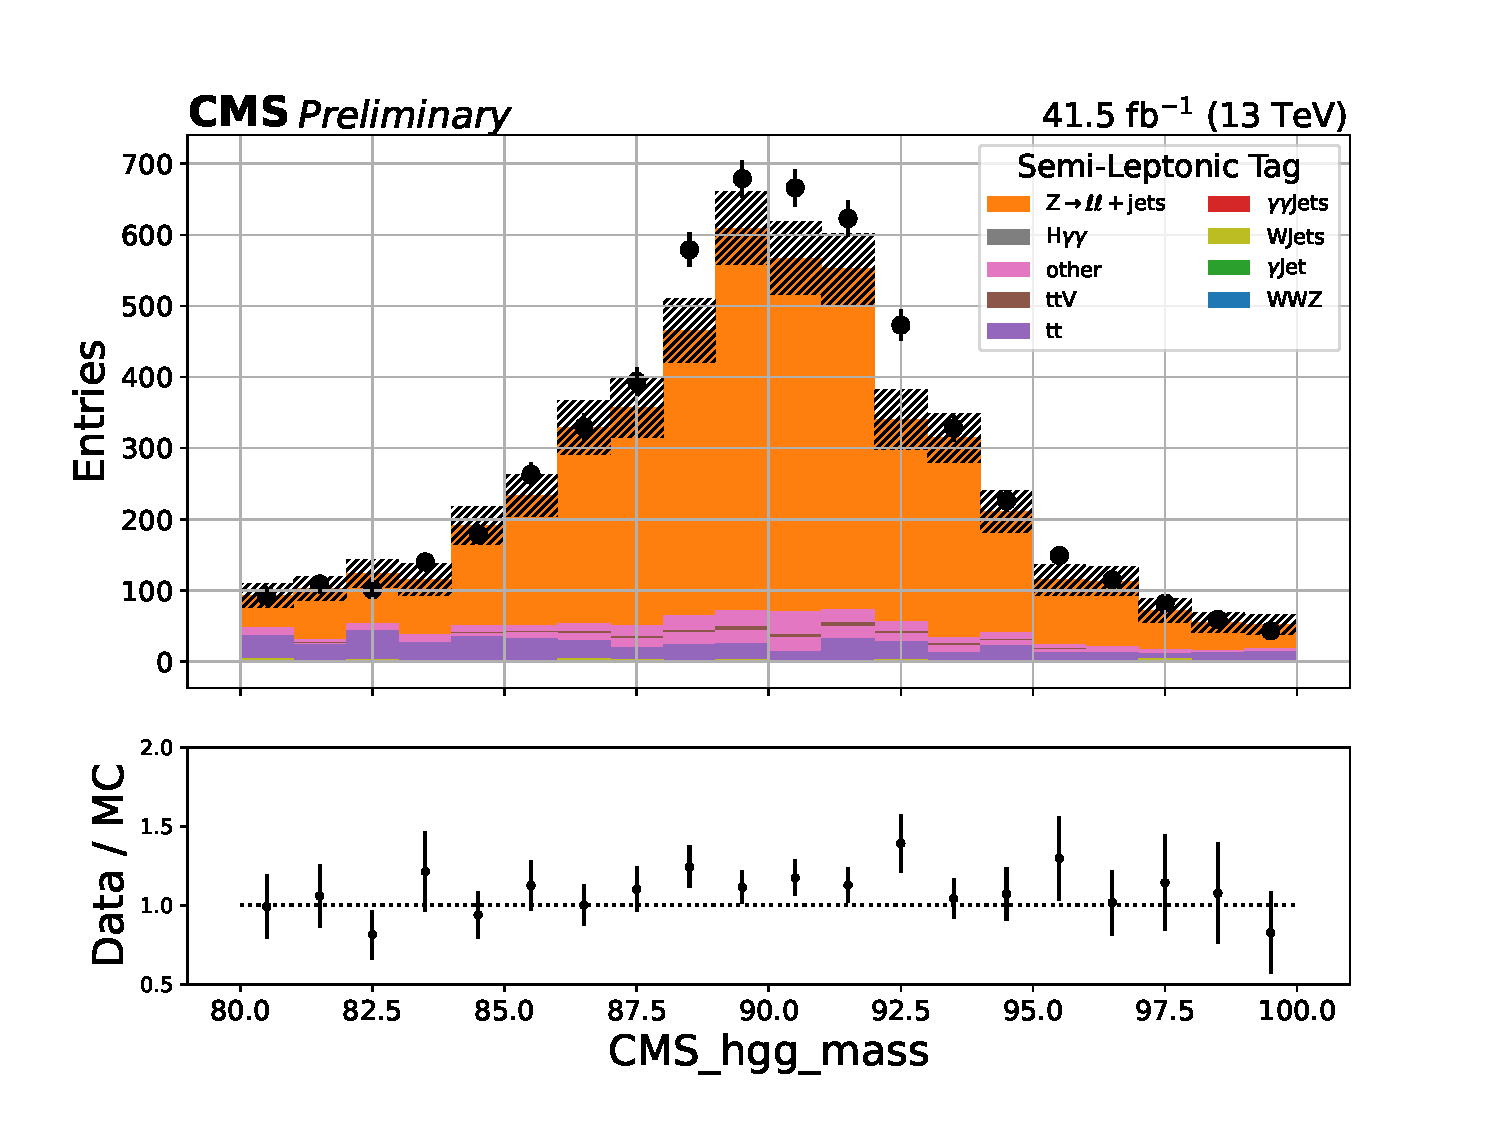
\includegraphics[width=0.45\textwidth]{Sections/HHWWgg/images/DNN_andSignal_Validation/nonlog/CMS_hgg_mass_HHWWggTag_0.pdf}}
    \qquad
    \subfloat[Logarithmic y scale]{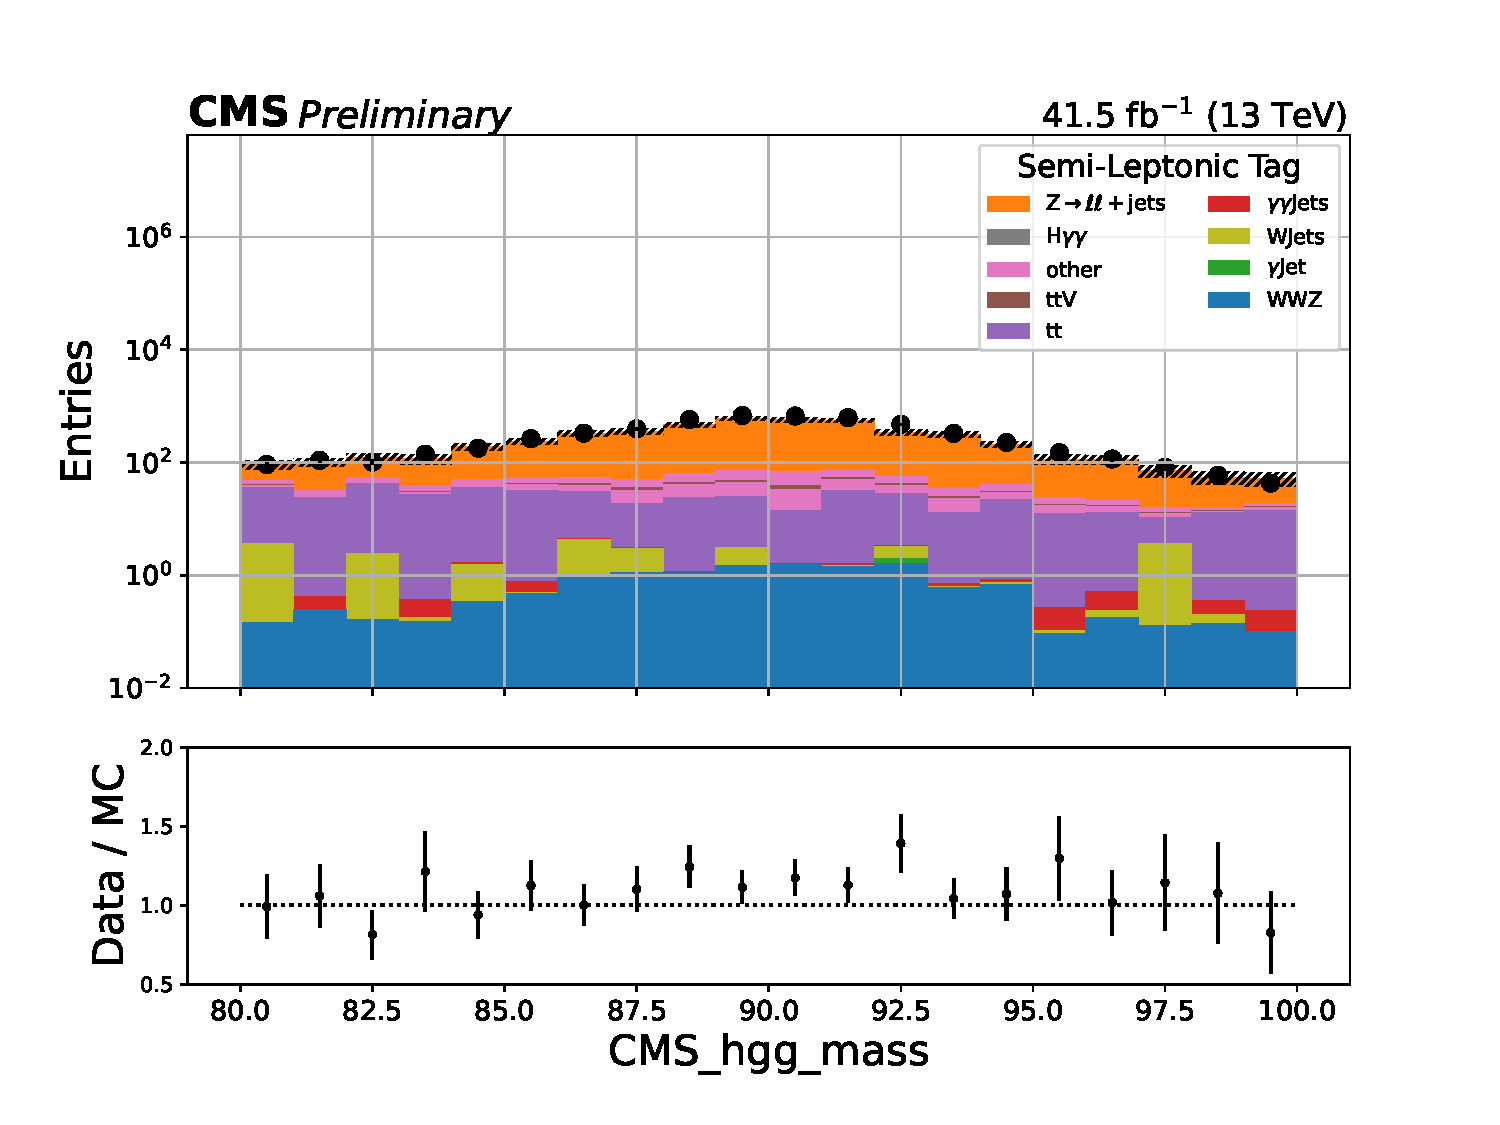
\includegraphics[width=0.45\textwidth]{Sections/HHWWgg/images/DNN_andSignal_Validation/log/CMS_hgg_mass_HHWWggTag_0.pdf}}
    \caption{Semileptonic category: Di-electron mass in the above defined control region, shown in linear and logarithmic y scale. \label{fig:SL_diEleMass}
    }
\end{figure} 

% \begin{figure}[!h]
%     \setcounter{subfigure}{0}
%     \centering
%     \subfloat[Linear y scale]{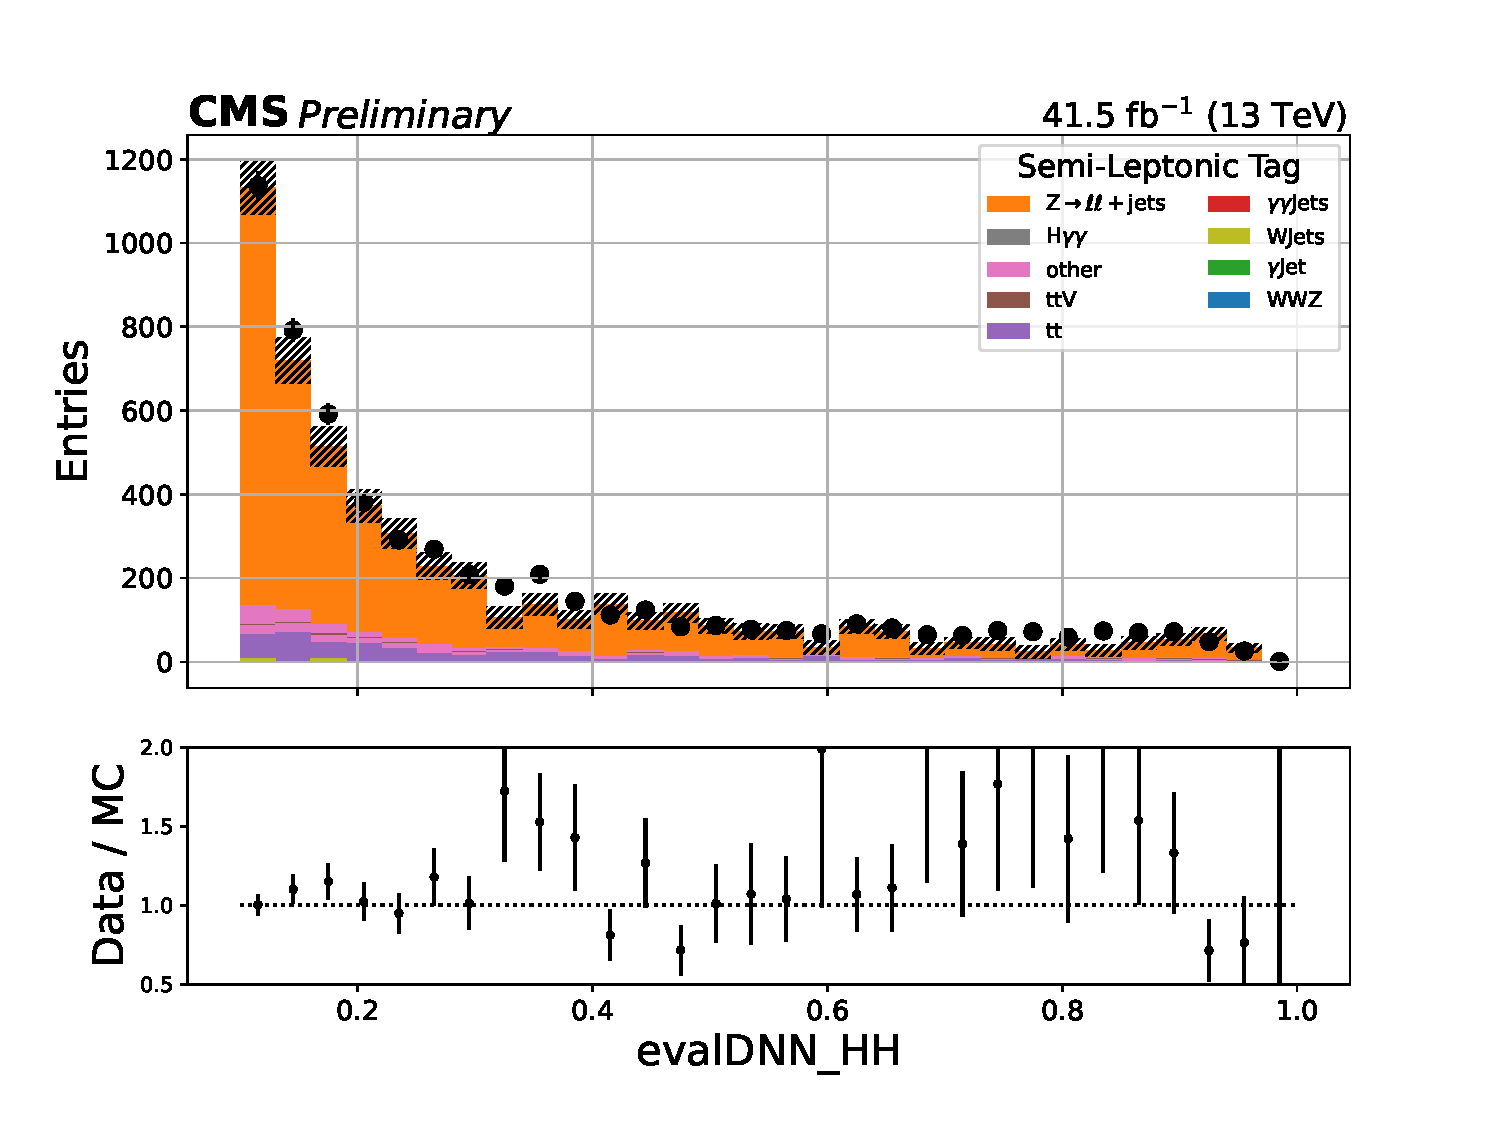
\includegraphics[width=0.45\textwidth]{Sections/HHWWgg/images/DNN_andSignal_Validation/nonlog/evalDNN_HH_HHWWggTag_0.pdf}}
%     \qquad
%     \subfloat[Logarithmic y scale]{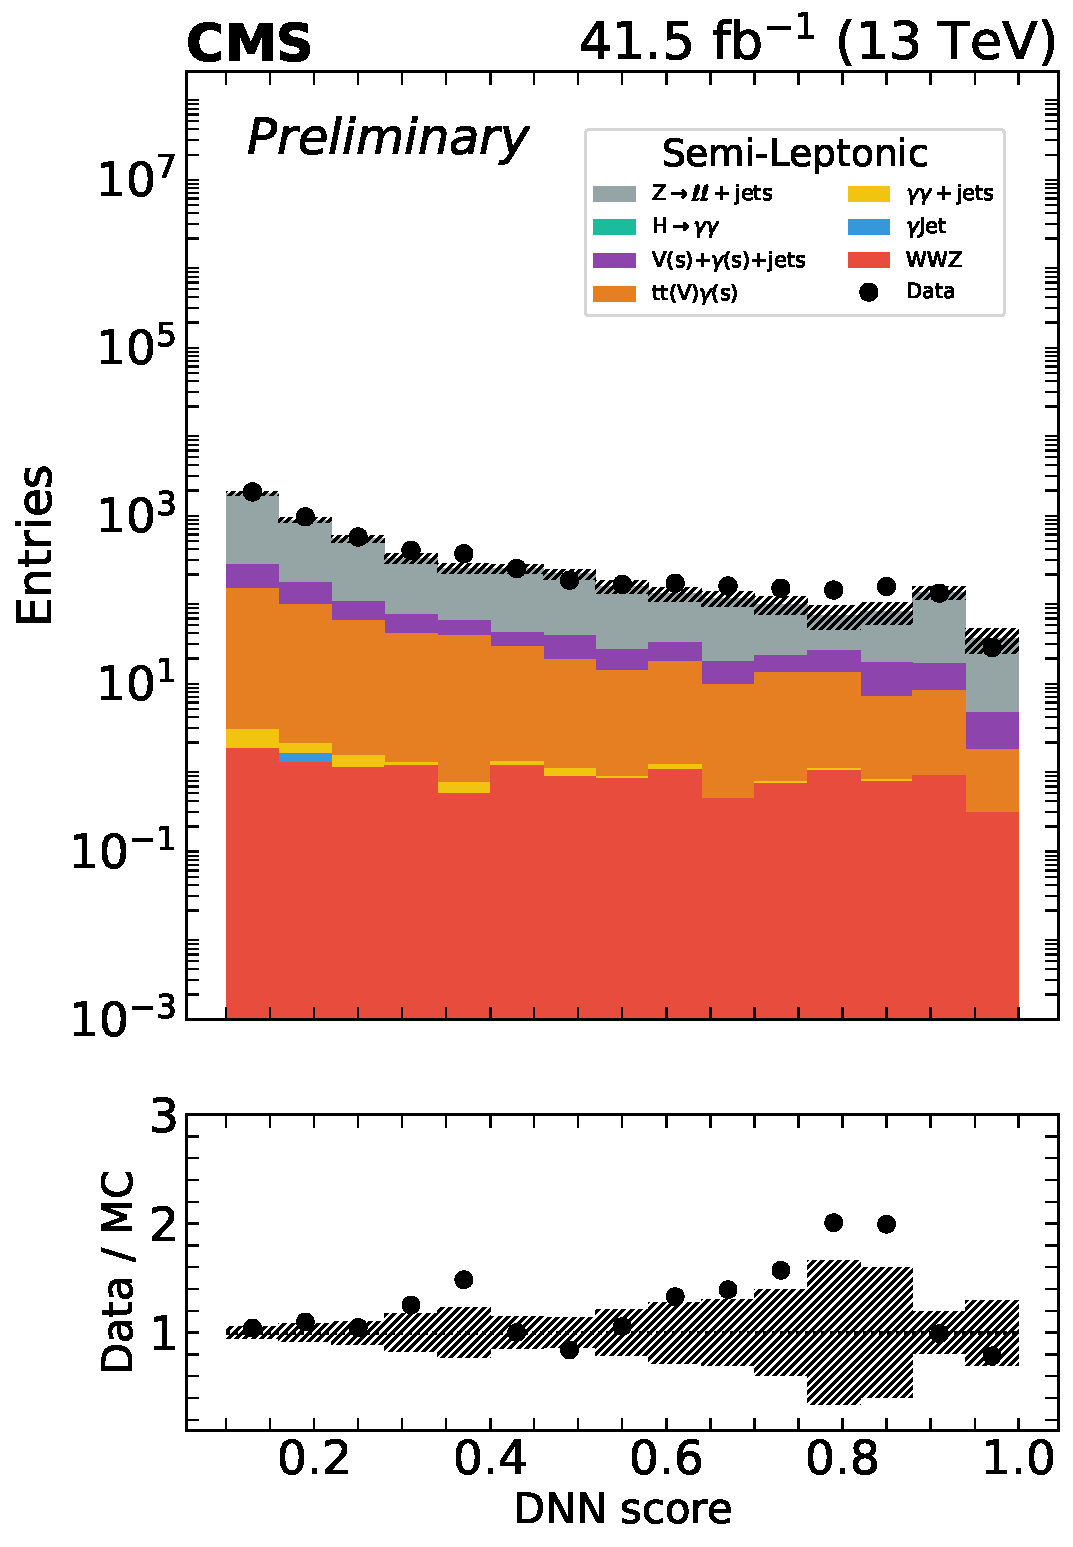
\includegraphics[width=0.45\textwidth]{Sections/HHWWgg/images/DNN_andSignal_Validation/log/evalDNN_HH_HHWWggTag_0.pdf}}
%     \caption{Semileptonic category: Semileptonic DNN score in the above defined control region. \label{fig:SL_DNN_CR}
%     }
% \end{figure}

\begin{figure}[h!]
    \centering
    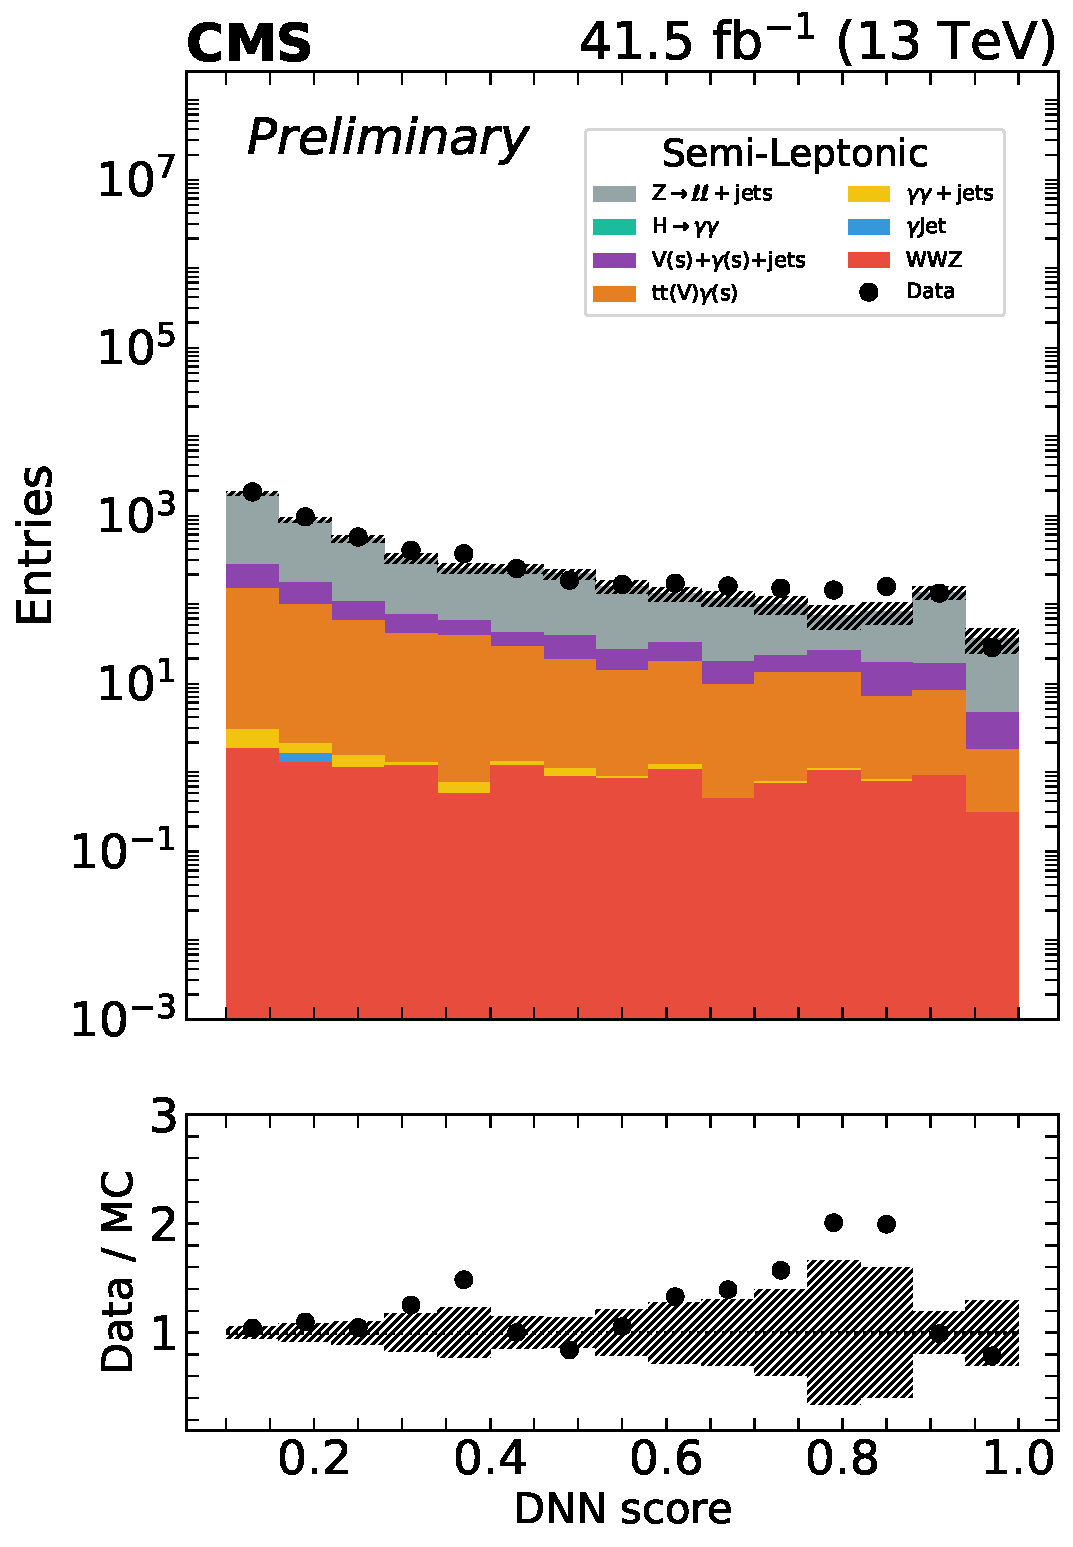
\includegraphics[width=0.45\textwidth]{Sections/HHWWgg/images/DNN_andSignal_Validation/log/evalDNN_HH_HHWWggTag_0.pdf}
    \caption{Semileptonic category: Semileptonic DNN score in the above defined control region. \label{fig:SL_DNN_CR}}
\end{figure}

\begin{figure}[!h]
    \setcounter{subfigure}{0}
    \centering
    \subfloat[Scaled Leading Photon pt $>$ 0]{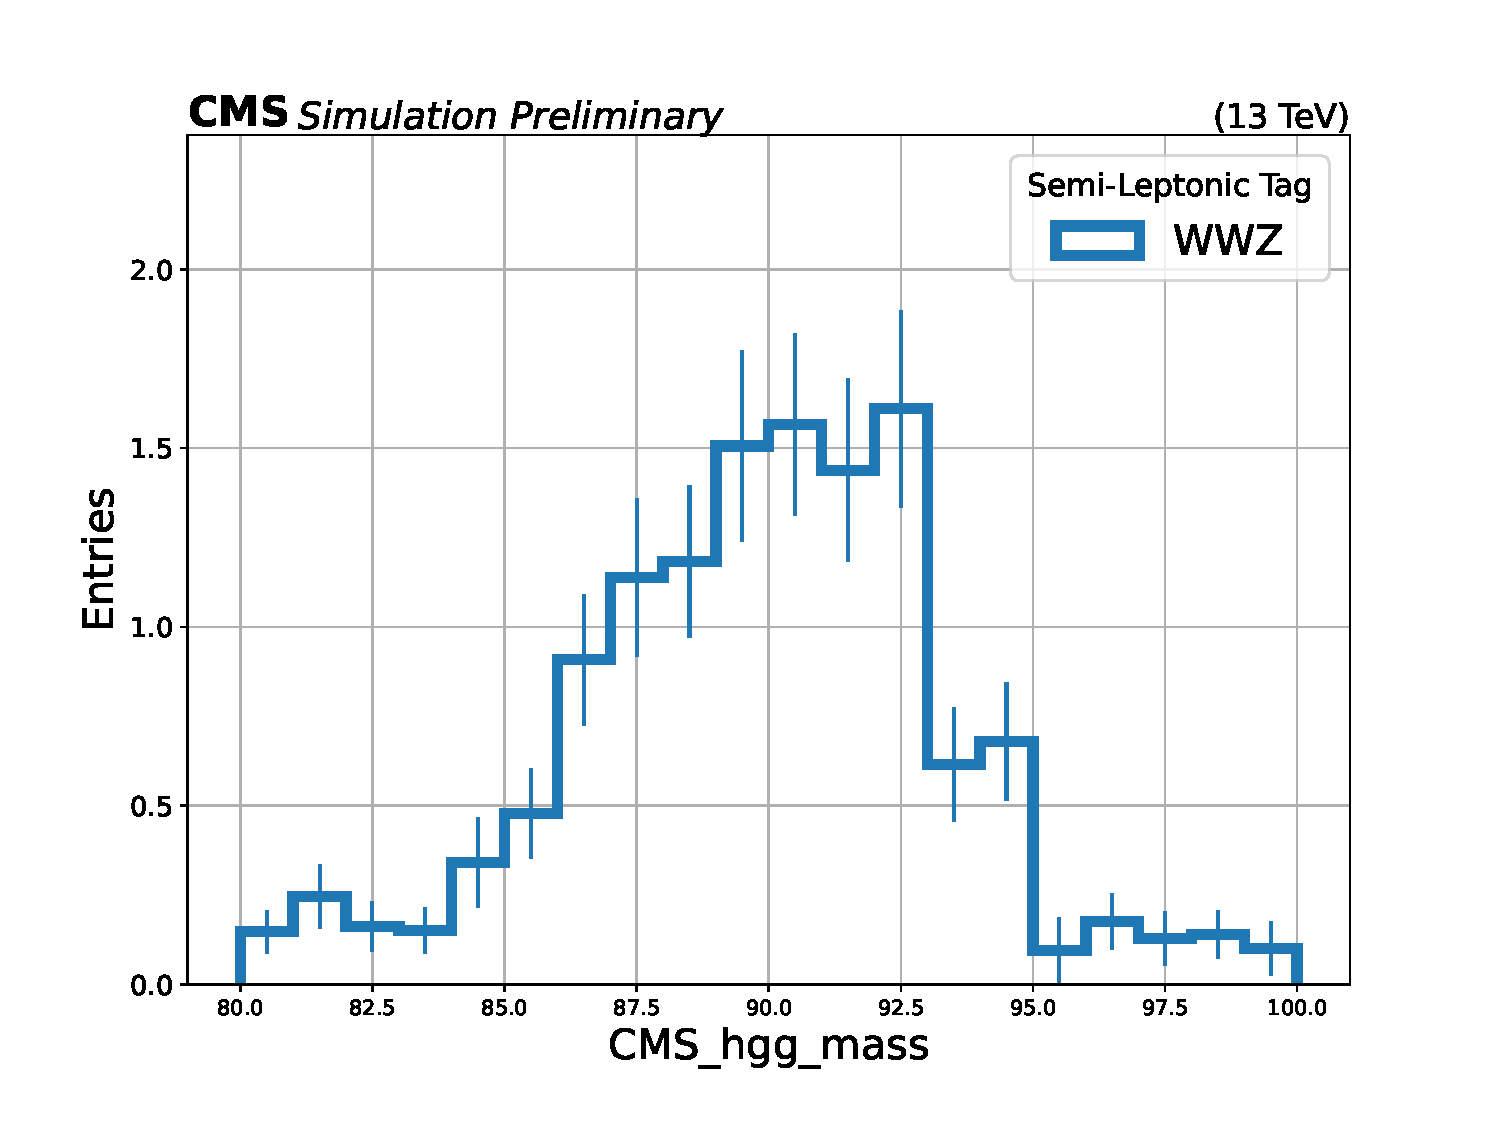
\includegraphics[width=0.45\textwidth]{Sections/HHWWgg/images/DNN_andSignal_Validation/nonlog/WWZonly_Scaled_Leading_Photon_pt_CUT_0_CMS_hgg_mass_HHWWggTag_0.pdf}}
    \qquad
    \subfloat[Scaled Leading Photon pt $>$ 1.0]{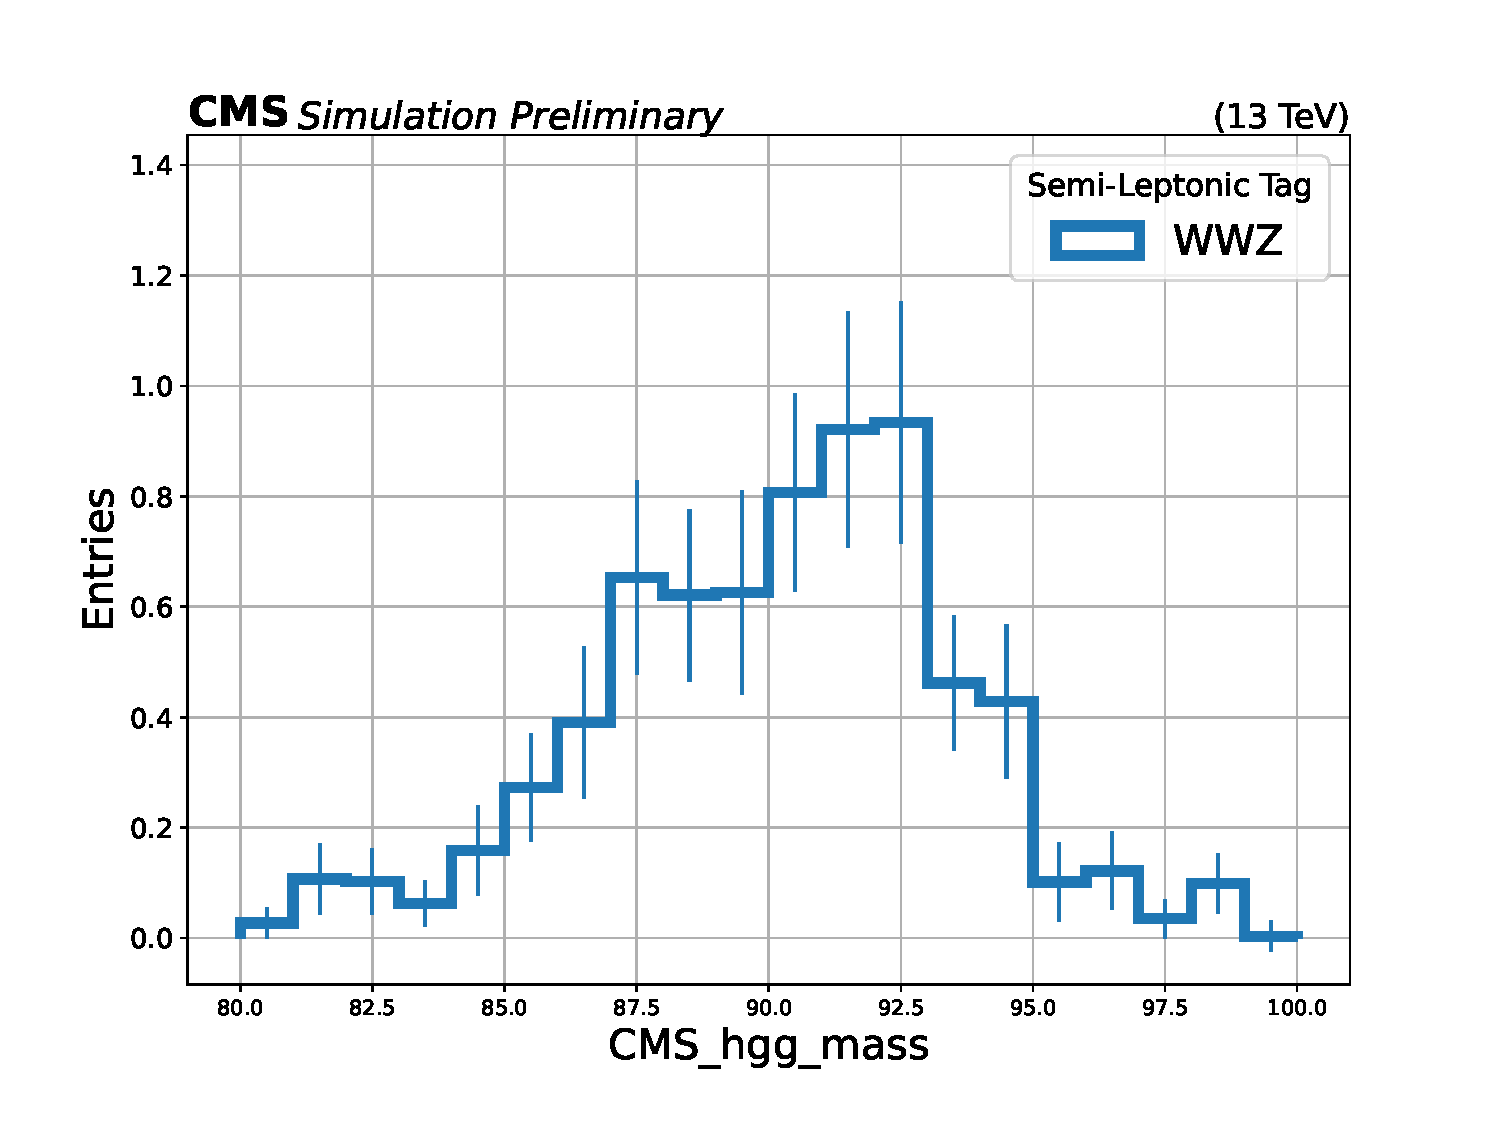
\includegraphics[width=0.45\textwidth]{Sections/HHWWgg/images/DNN_andSignal_Validation/nonlog/WWZonly_Scaled_Leading_Photon_pt_CUT_1_CMS_hgg_mass_HHWWggTag_0.pdf}}
    \caption{Semileptonic category: Di-electron mass of the WWZ process with and without a scaled leading photon pt selection of 1.0 applied. \label{fig:SL_diEleMass_WWZ}
    }
\end{figure}

\begin{figure}[!h]
    \setcounter{subfigure}{0}
    \centering
    \subfloat[Scaled Leading Photon pt $>$ 0]{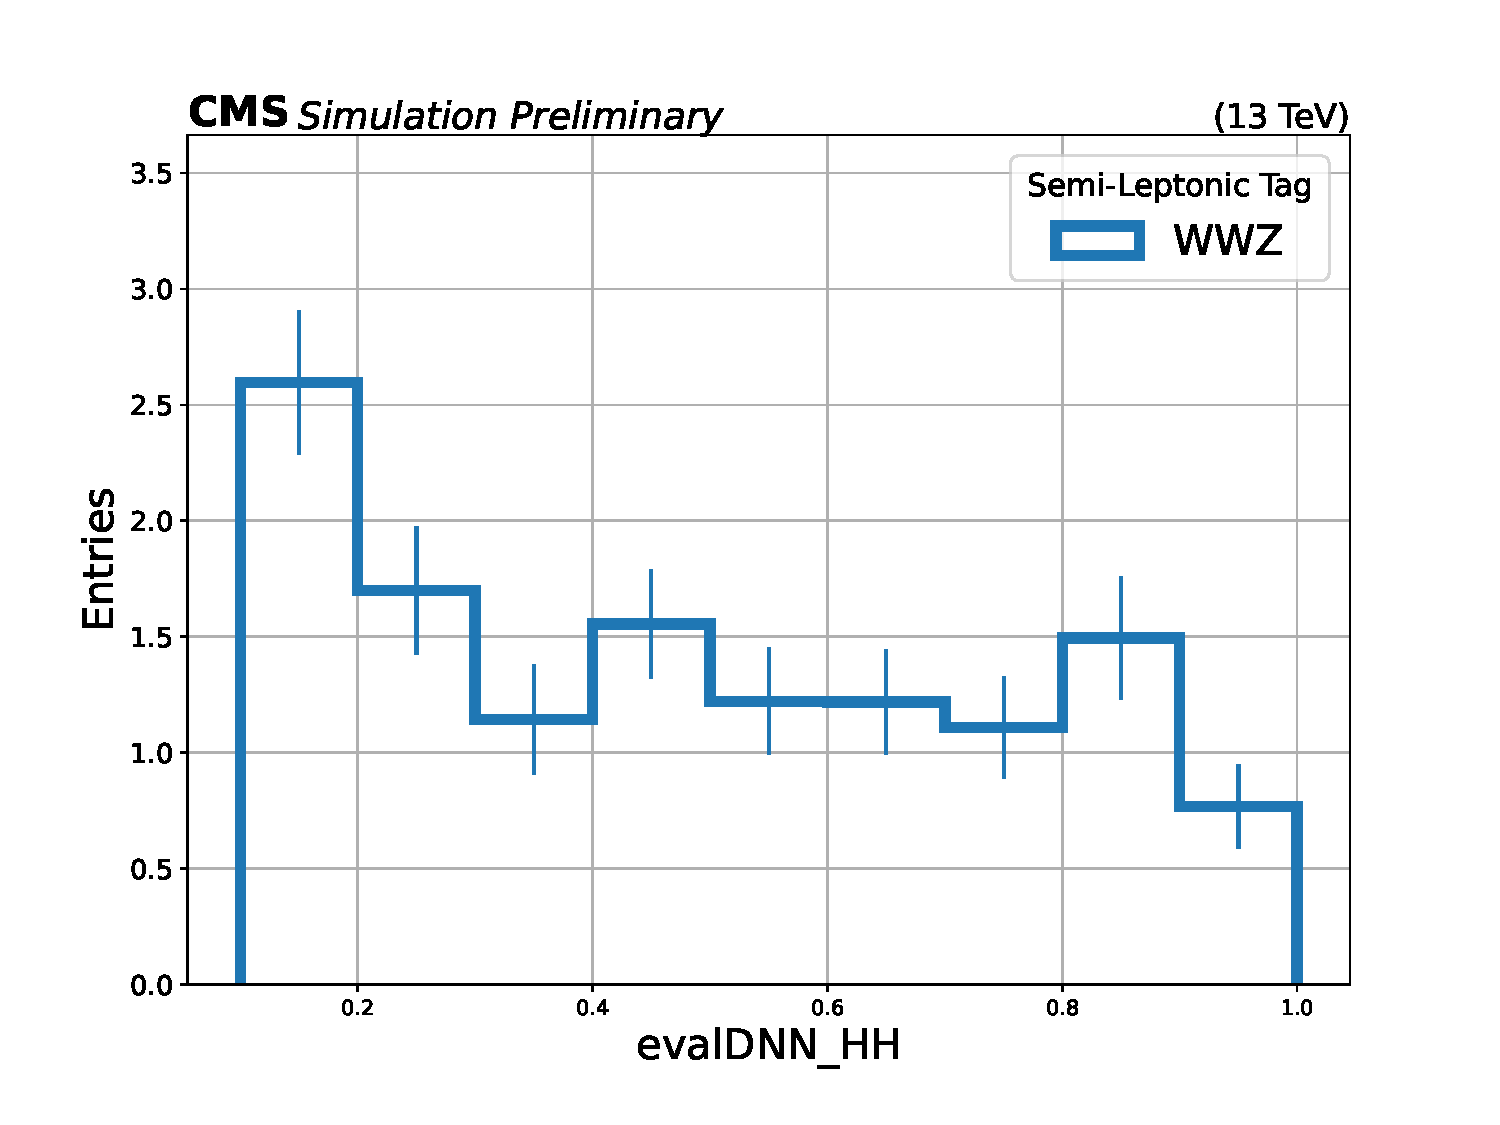
\includegraphics[width=0.45\textwidth]{Sections/HHWWgg/images/DNN_andSignal_Validation/nonlog/WWZonly_Scaled_Leading_Photon_pt_CUT_0_evalDNN_HH_HHWWggTag_0.pdf}}
    \qquad
    \subfloat[Scaled Leading Photon pt $>$ 1.0]{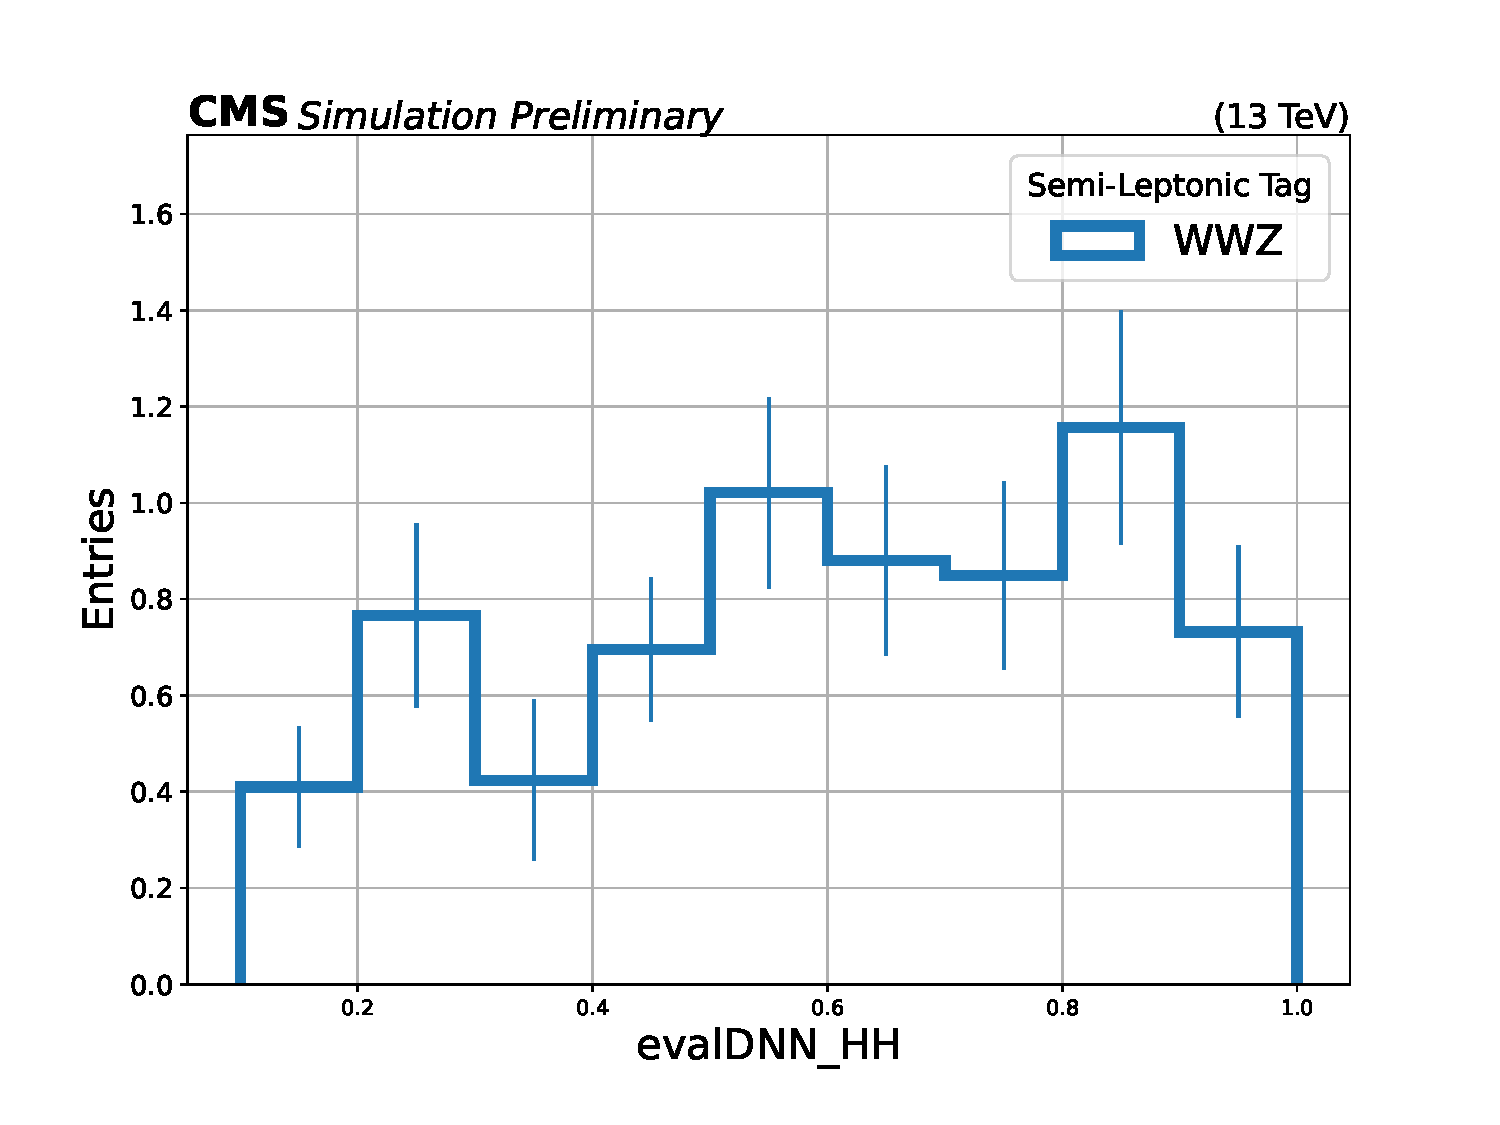
\includegraphics[width=0.45\textwidth]{Sections/HHWWgg/images/DNN_andSignal_Validation/nonlog/WWZonly_Scaled_Leading_Photon_pt_CUT_1_evalDNN_HH_HHWWggTag_0.pdf}}
    \caption{Semileptonic category: DNN score of the WWZ process with and without a scaled leading photon pt selection of 1.0 applied. \label{fig:SL_DNNscore_WWZ}
    }
\end{figure}


\begin{figure}[!h]
    \setcounter{subfigure}{0}
    \centering
    \subfloat[Linear y scale]{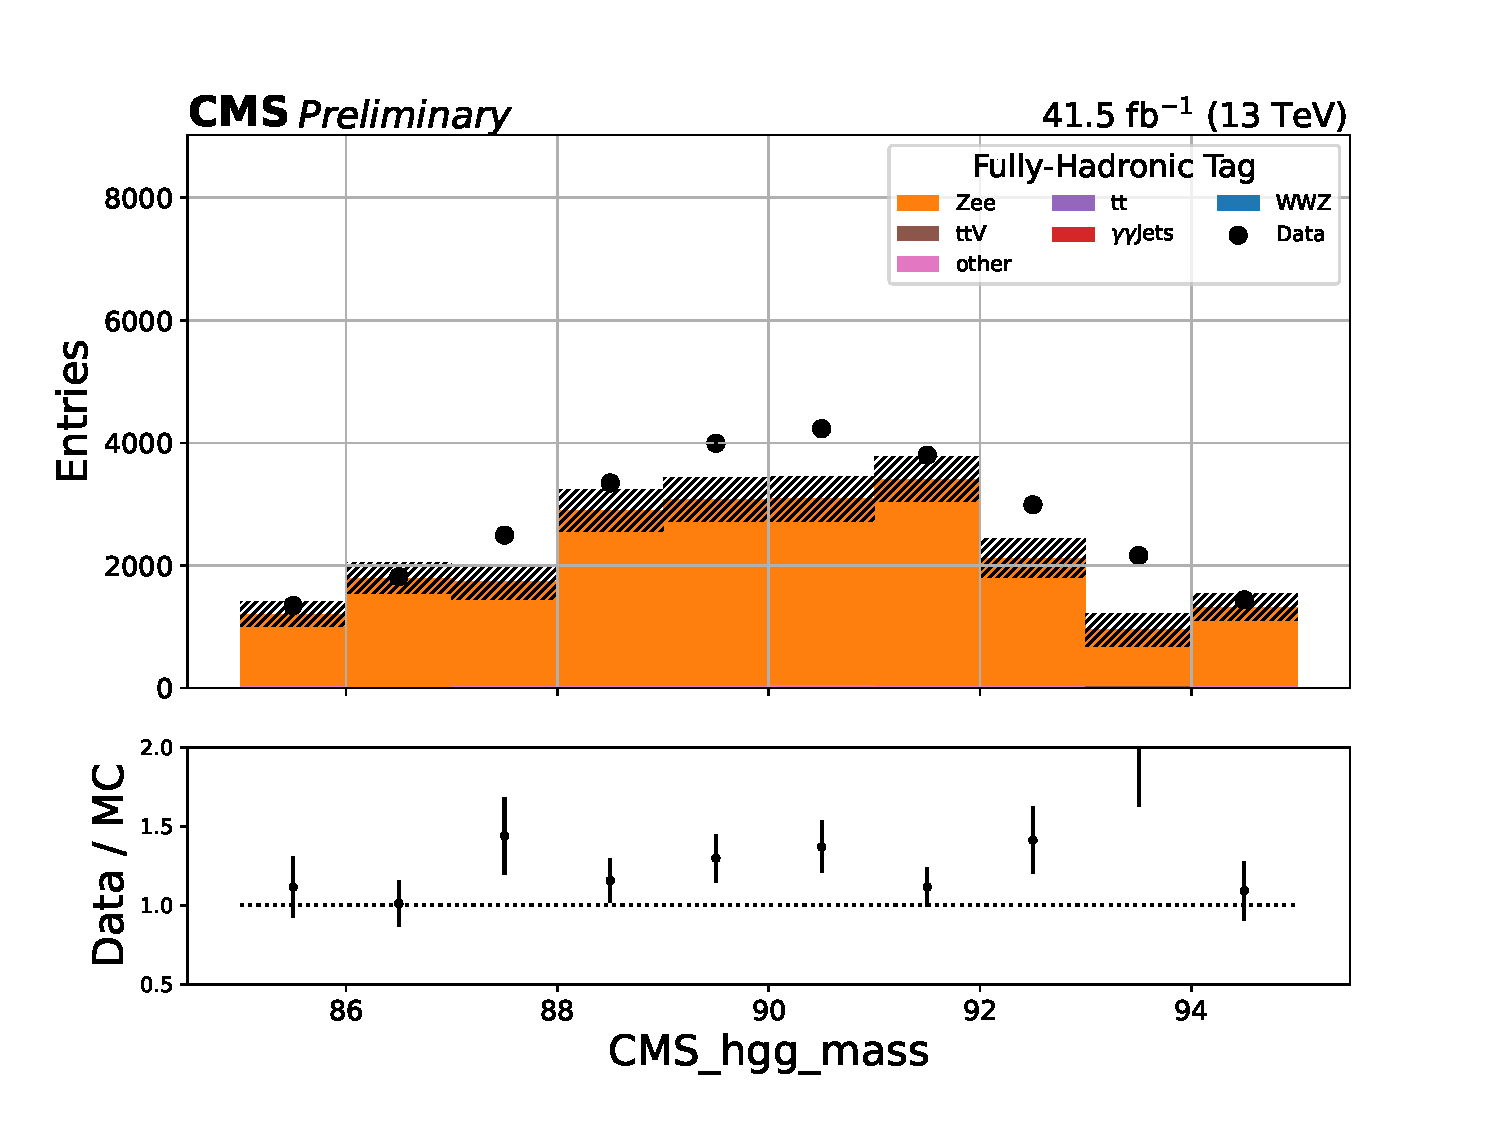
\includegraphics[width=0.45\textwidth]{Sections/HHWWgg/images/DNN_andSignal_Validation/fullyhadronic/CMS_hgg_mass_HHWWggTag_1_nonLog.pdf}}
    \qquad
    \subfloat[Logarithmic y scale]{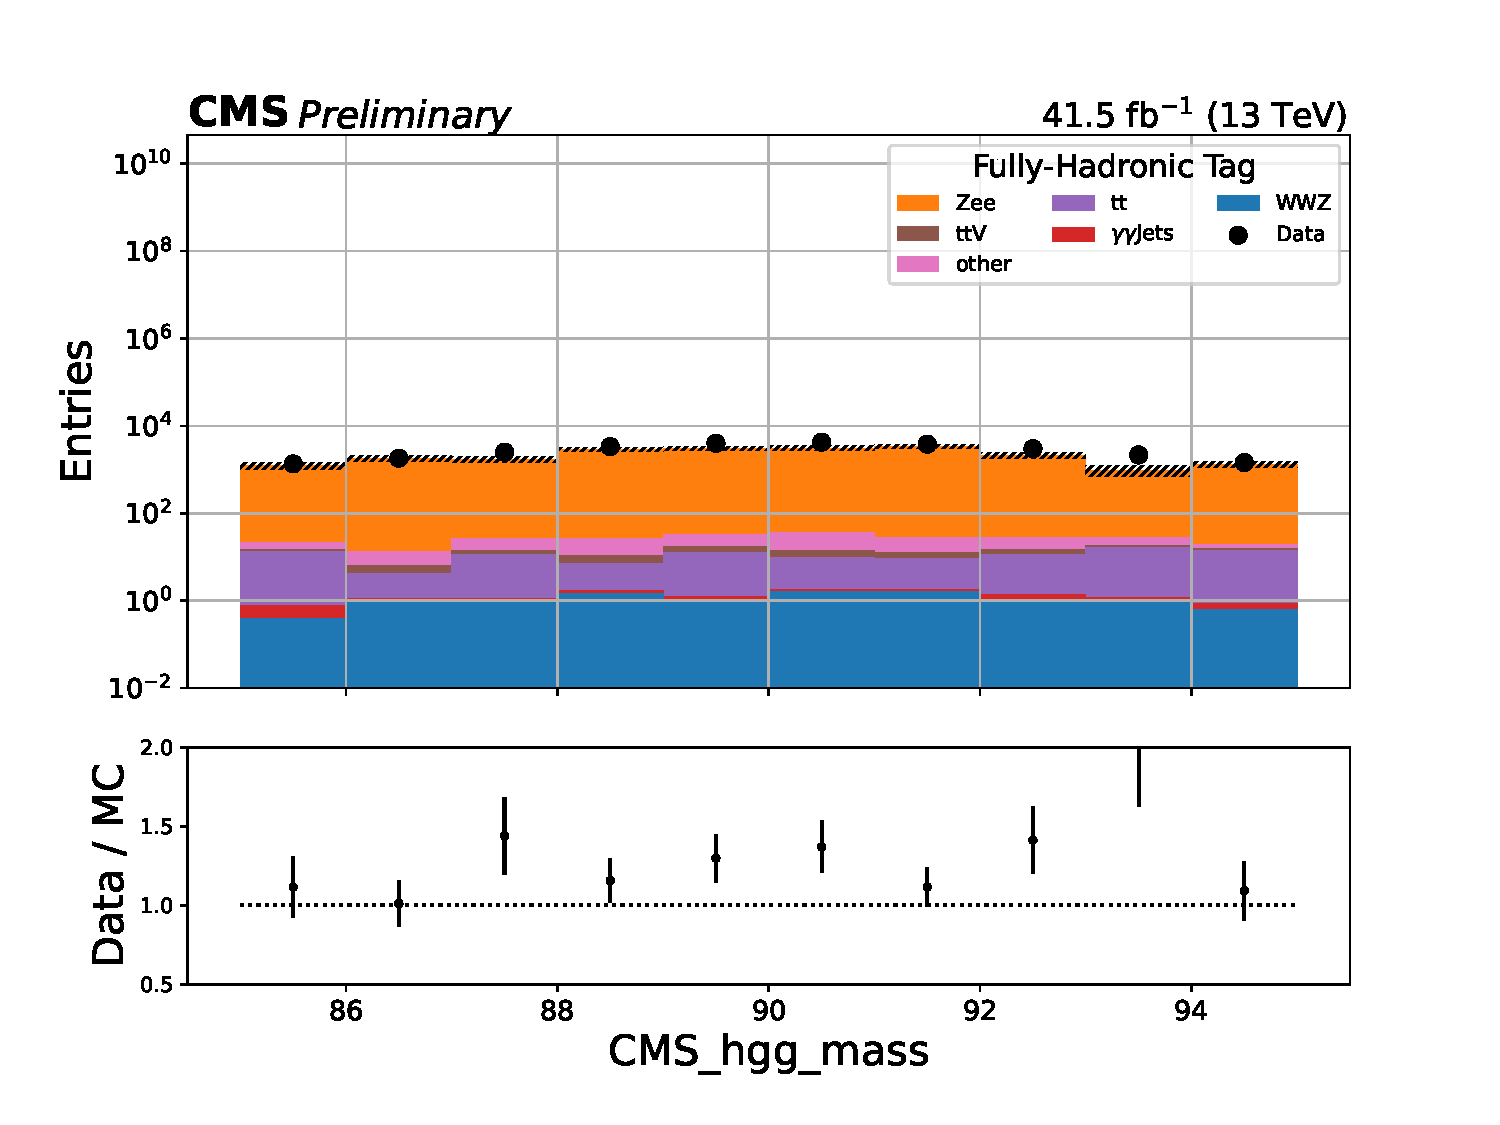
\includegraphics[width=0.45\textwidth]{Sections/HHWWgg/images/DNN_andSignal_Validation/fullyhadronic/CMS_hgg_mass_HHWWggTag_1_log.pdf}}
    \caption{Fullyhadronic category: Di-electron mass in the above defined control region, shown in linear and logarithmic y scale. \label{fig:FH_diEleMass}
    }
\end{figure}

% \begin{figure}[!h]
%     \setcounter{subfigure}{0}
%     \centering
%     \subfloat[Linear y scale]{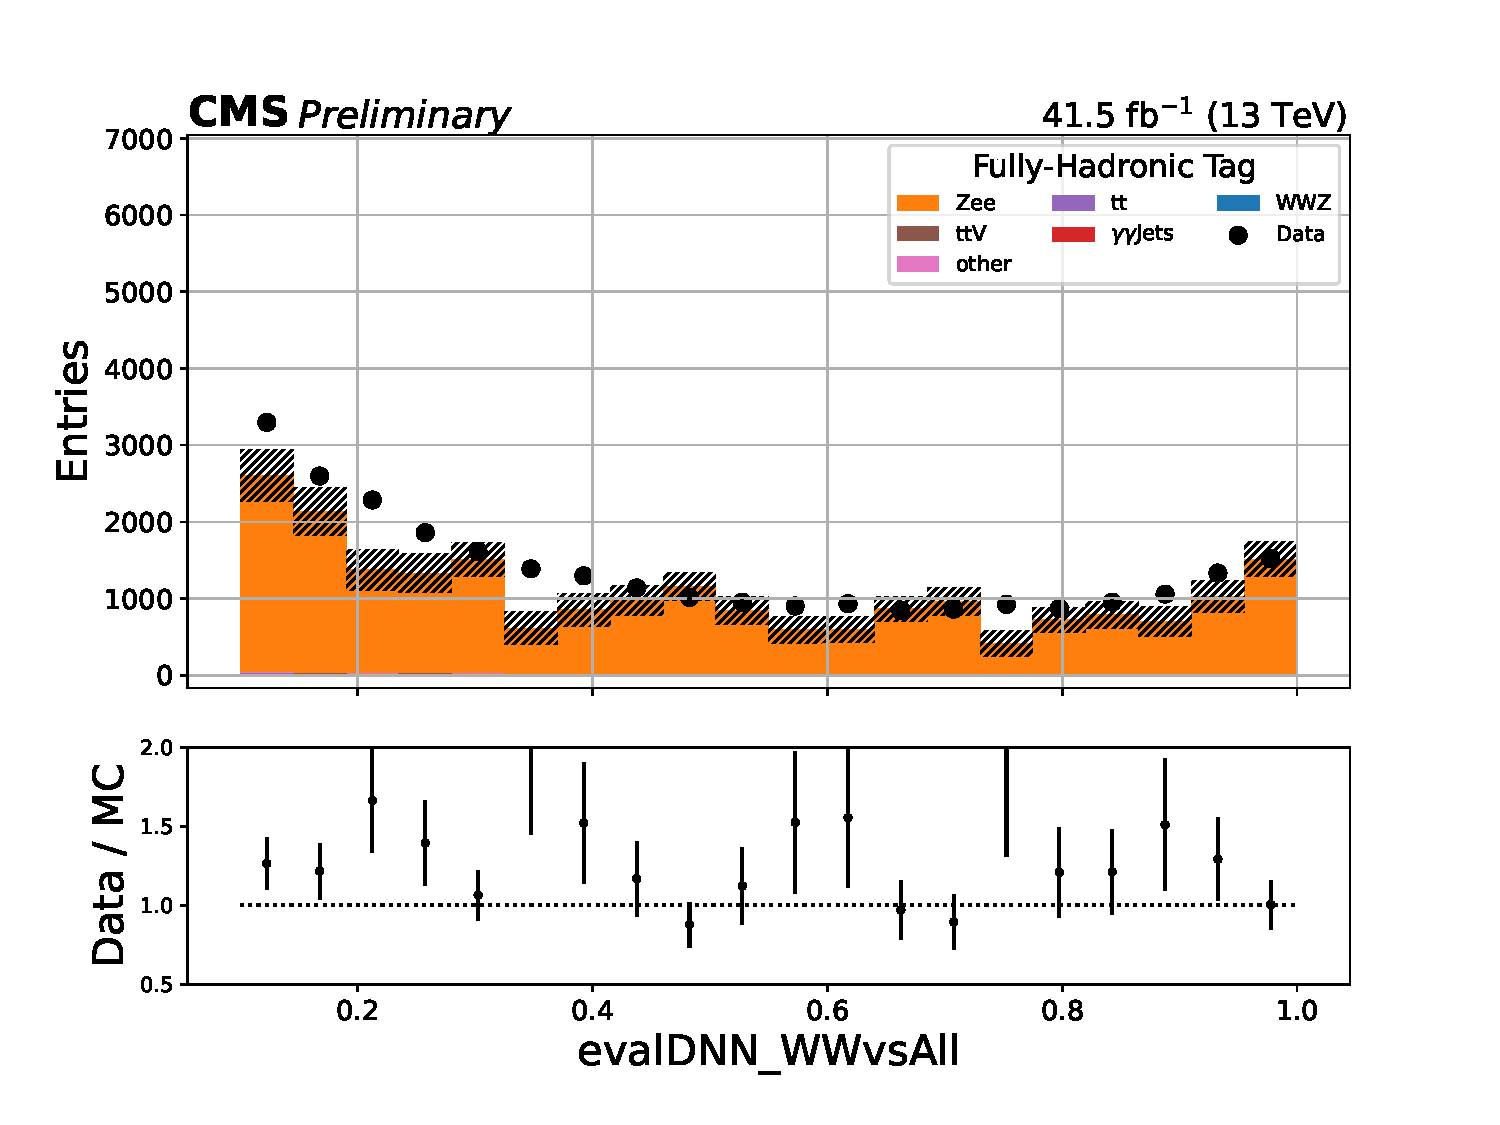
\includegraphics[width=0.45\textwidth]{Sections/HHWWgg/images/DNN_andSignal_Validation/fullyhadronic/evalDNN_WWvsAll_HHWWggTag_1_nonLog.pdf}}
%     \qquad
%     \subfloat[Logarithmic y scale]{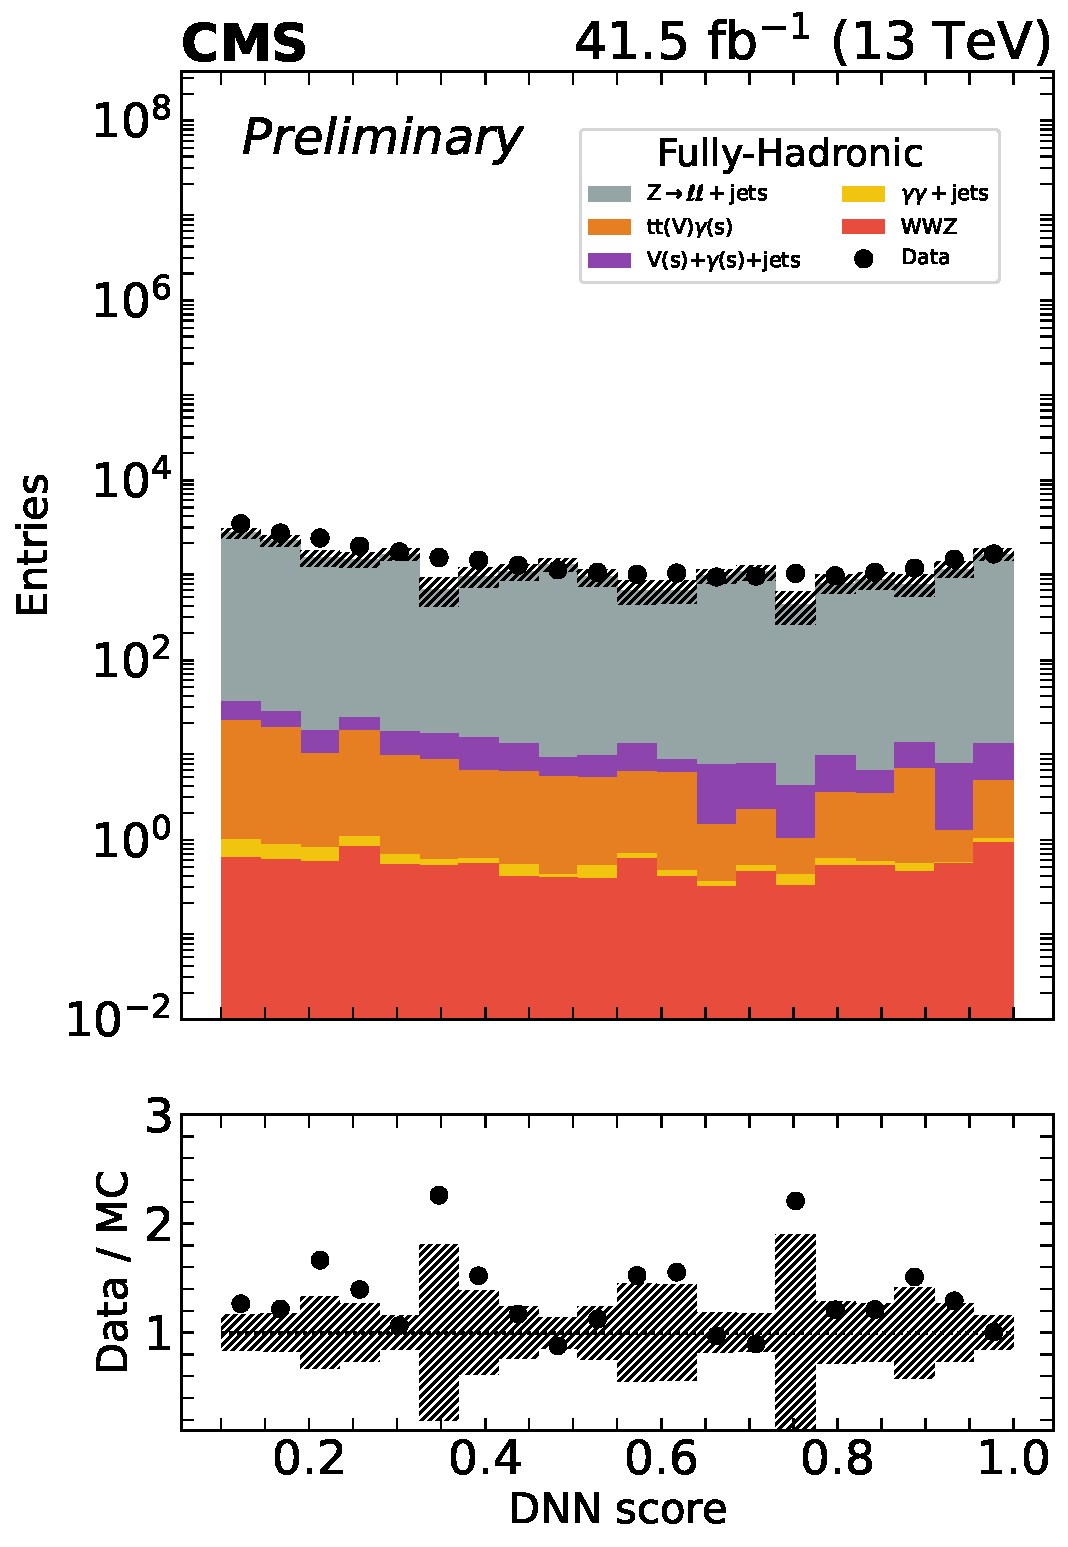
\includegraphics[width=0.45\textwidth]{Sections/HHWWgg/images/DNN_andSignal_Validation/fullyhadronic/evalDNN_WWvsAll_HHWWggTag_1_log.pdf}}
%     \caption{Fullyhadronic category: Fullyhadronic DNN score in the above defined control region, shown in linear and logarithmic y scale. \label{fig:FH_DNN_Score} 
%     }
% \end{figure}

\begin{figure}[h!]
    \centering
    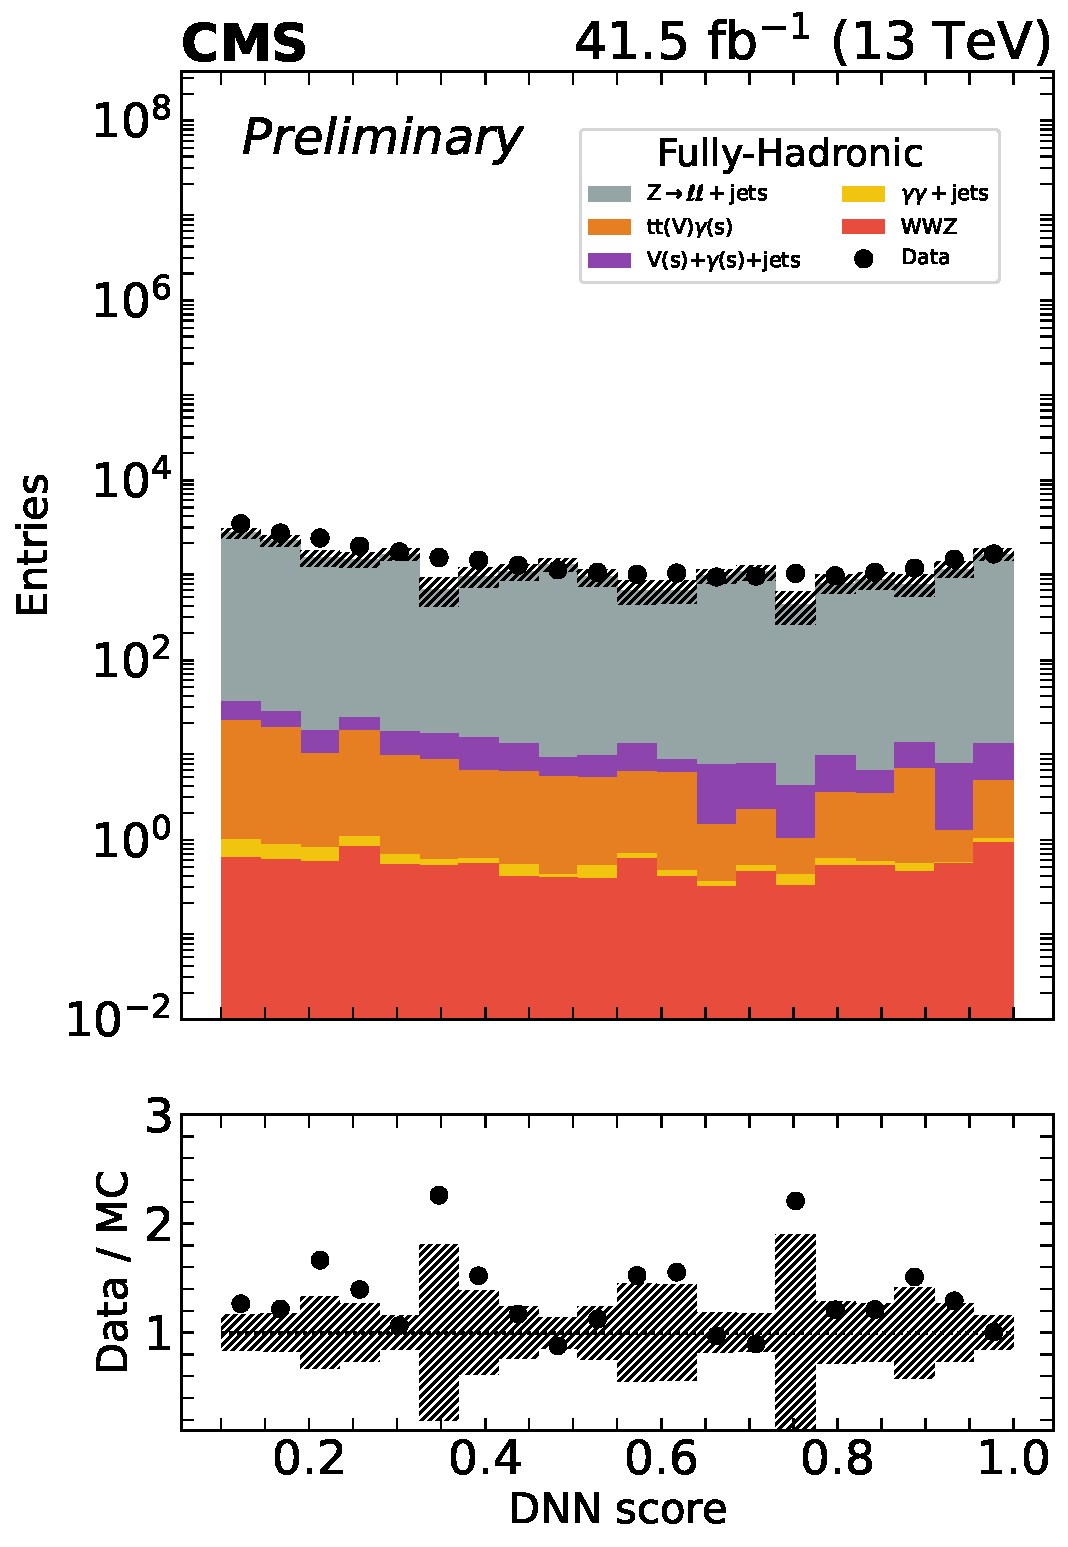
\includegraphics[width=0.45\textwidth]{Sections/HHWWgg/images/DNN_andSignal_Validation/fullyhadronic/evalDNN_WWvsAll_HHWWggTag_1_log.pdf}
    \caption{Fullyhadronic category: Fullyhadronic DNN score in the above defined control region. \label{fig:FH_DNN_Score} }
\end{figure}

\begin{figure}[!h]
    \setcounter{subfigure}{0}
    \centering
    \subfloat[WWZ di-electron mass]{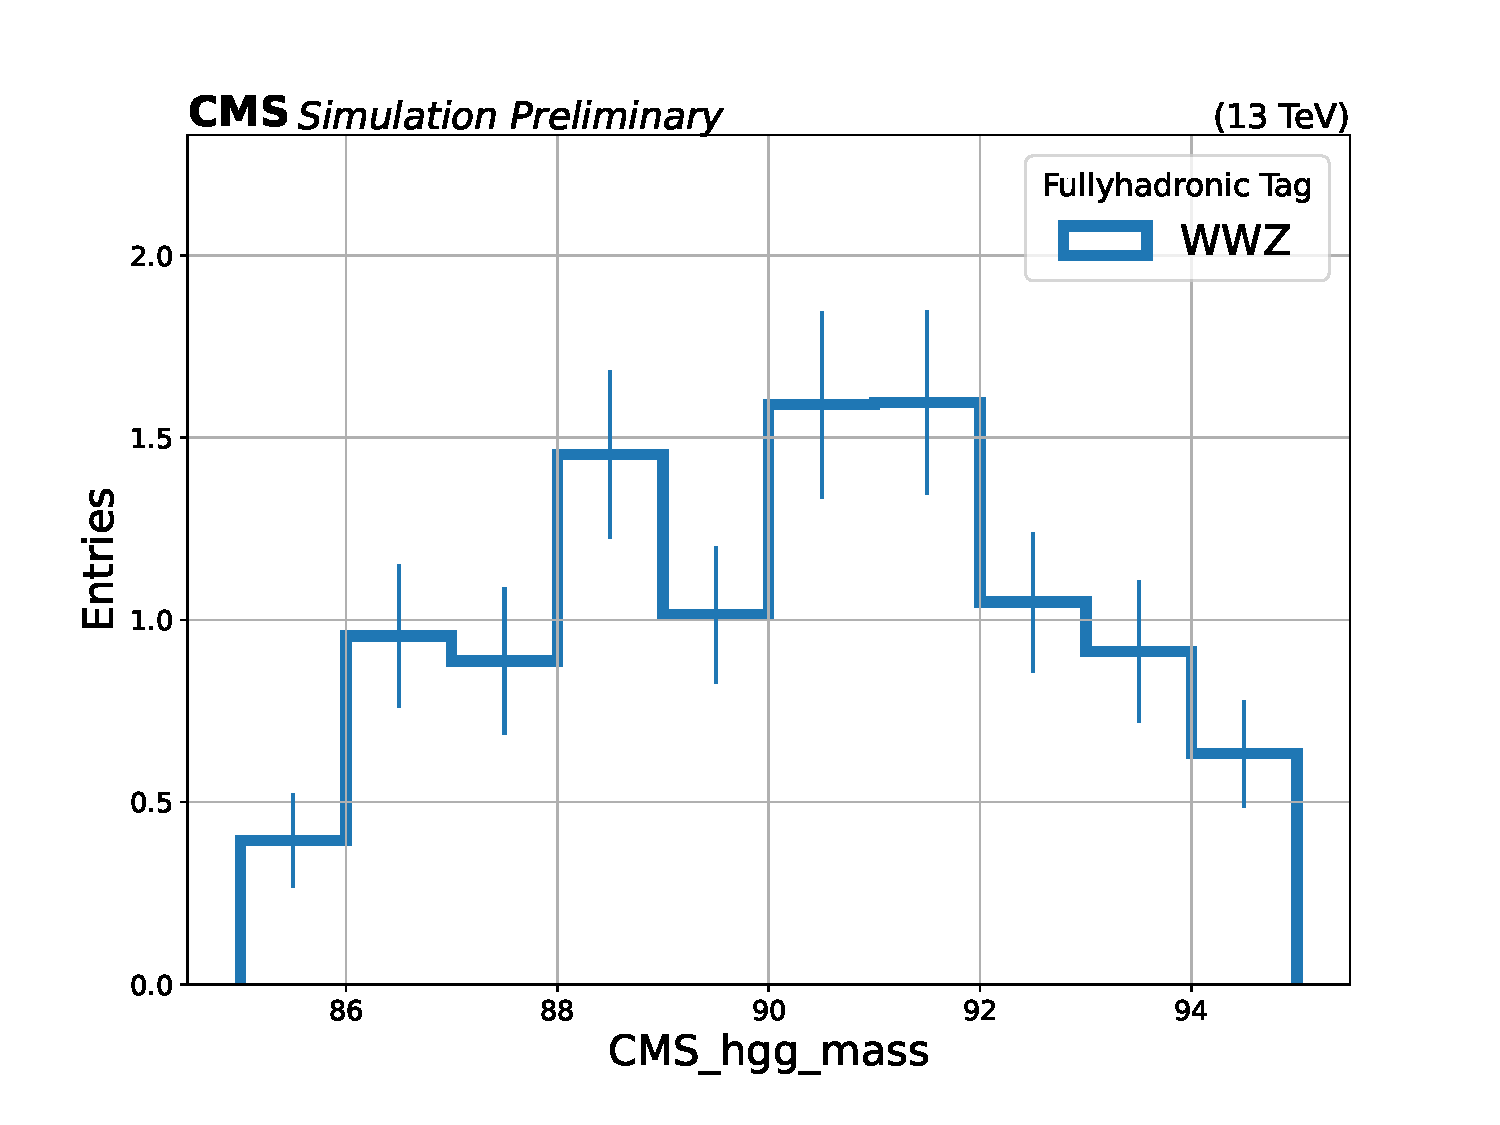
\includegraphics[width=0.45\textwidth]{Sections/HHWWgg/images/DNN_andSignal_Validation/fullyhadronic/WWZonly_CMS_hgg_mass_HHWWggTag_1.pdf}}
    \qquad
    \subfloat[WZZ DNN score]{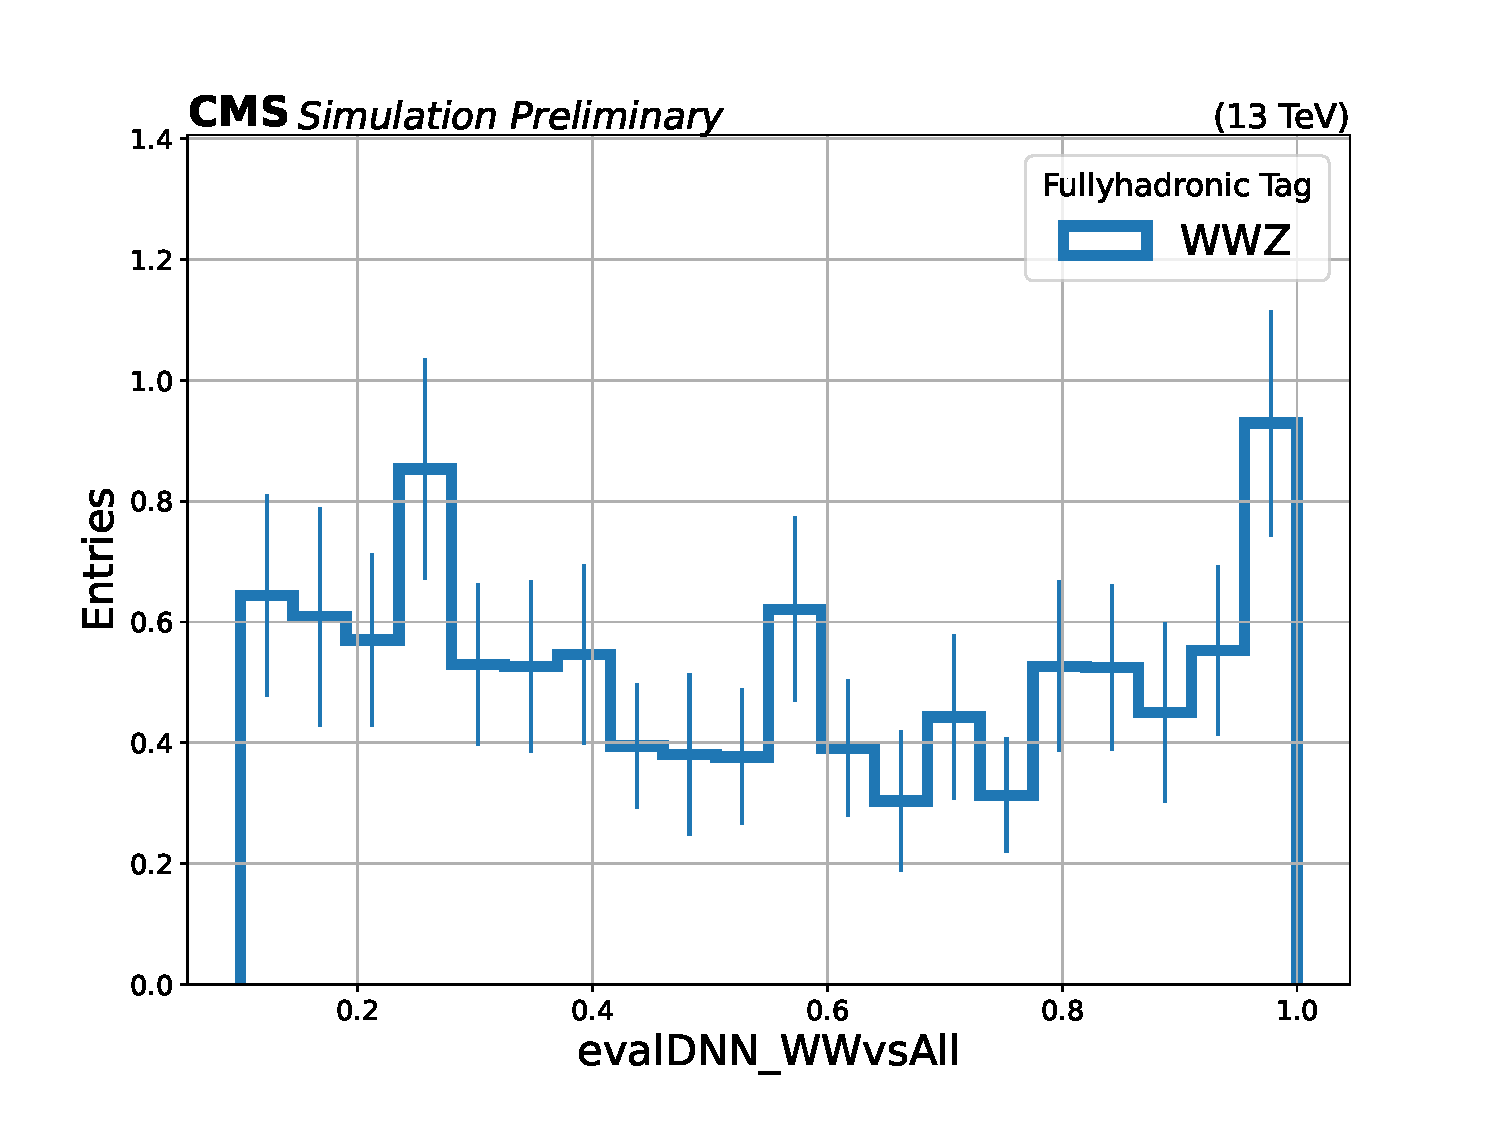
\includegraphics[width=0.45\textwidth]{Sections/HHWWgg/images/DNN_andSignal_Validation/fullyhadronic/WWZonly_evalDNN_WWvsAll_HHWWggTag_1.pdf}}
    \caption{Fullyhadronic category: Di-electron mass and fullyhadronic DNN score of the WWZ process. \label{fig:FH_WWZ}
    }
\end{figure}
